\documentclass[12pt,a4paper, titlepage, oneside]{article}

\usepackage{geometry}
\usepackage{amsmath}
\usepackage{graphicx}
\usepackage[backend=biber]{biblatex}
\usepackage{hyperref}

%bibliografia
\addbibresource{Spettroscopia.Bibliografia.bib}

%intestazione
\title{Spettroscopia}
\author{Riccardo Peltretti}
\date{\today}

\begin{document}
    \maketitle
    
    \begin{abstract}
        La spettroscopia è la branca della fisica ottica che si occupa di studiare gli spettri elettromagnetici, ovvero la composizione della luce, prodotti dalle diverse sostanze, per identificarle o osservarne alcune proprietà. L'origine della spettroscopia moderna una branca della scienza che ha origine nel 17° secolo con gli esperimenti di ottica di Isaac Newton (1666-1672), sebbene altri scenziati avessero precedentemente studiato lo spettro solare.\\
        Agli inizi del 19° secolo, grazie agli esperimenti di Joseph von Fraunhofer, la spettroscopia è diventata una tecnica più precisa e scientifica, rivelandosi di fondamentale importanza per la fisica, la chimica e l'astronomia. 
    \end{abstract}

    \tableofcontents
    \clearpage

    \section{Storia}
    Tradizionalmente si fa iniziare la spettroscopia, con le prime osservazioni effettuate da \href{https://it.wikipedia.org/wiki/Isaac_Newton}{Isaac Newton}, tra il 1666 ed il 1672, della \href{https://it.wikipedia.org/wiki/Dispersione_ottica}{dispersione cromatica} subita dalla luce attraverso un prisma \ref{fig:dispersione}.
    \begin{figure}[h!]
        \begin{center}
            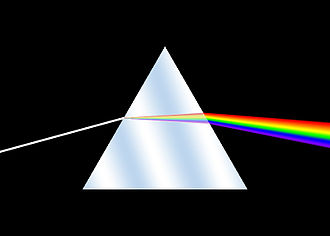
\includegraphics[width=175px, keepaspectratio]{media/dispersion_prism.jpg}
            \caption{L'indice di rifrazione di un \href{https://it.wikipedia.org/wiki/Prisma_triangolare}{prisma triangolare} dipende dalla lunghezza d'onda. Di conseguenza le componenti del fascio luminoso vengono rifratte ad angoli diversi, causandone la dispersione.}
        \end{center}
        \label{fig:dispersione}
    \end{figure}
    Newton raccolse le sue osservazioni ed i suoi esperimenti in un trattato, \href{https://it.wikipedia.org/wiki/Opticks}{\textbf{Opticks}}, di fondamentale per lo sviluppo dell'\href{https://it.wikipedia.org/wiki/Ottica_fisica}{ottica fisica}, tuttavia non fu il primo ad studiare le proprietà della luce.

    Già nella \href{https://it.wikipedia.org/wiki/Naturalis_historia}{\textbf{Historia Naturalis}} di \href{https://it.wikipedia.org/wiki/Plinio_il_Vecchio}{Plinio il Vecchio} troviamo alcuni riferimenti all'esistenza di pietre cerunie, o \href{https://it.wikipedia.org/wiki/Folgorite}{folgoriti}, aventi la capacità di proiettare i colori dell'arcobaleno sulle pareti vicine, quando colpite dalla luce del sole \cite{naturalisHistoria}.\\
    
    \clearpage

    \section{Fisica}
    lorem ipsum
    \clearpage

    \section{Tecniche e Applicazioni}
    lorem ipsum
    \clearpage

    \section{Curiosità}
    lorem ipsum
    \clearpage

    \printbibliography
    \clearpage

    
\end{document}